\chapter{Limite y Continuidad}
\section{Limite}

El limite es la mayor erramienta para poder analisar el comportamiento de las funciones. \\
En si se trata de observar a que valor se acerca la funcion cuando la evaluamos en valores proximos a un punto.
\subsubsection{Entorno}
Un entorno comprende los valores cercanos al un punto dado (centro). El entorno de radio $1$ de $3$ comprende el intervalo $[2,4]$ o los valores de $x$ que cumplen con $1 \geq x \geq 3$ lo que notaremos $E(a)$, siendo $a$ el centro.\\
Tememos otros tipos de entornos ya sea a derecha o izquierda los cuales podemos describirlos con $r \geq x \geq a$ o $a \leq x leq r$, respectivamente (siendo $r$ el radio y a el centro). Y existe pa posobilidad de excluir el centro del entorno osea $ 0<|a-x|\leq$, lo cual notaremos con  $\stackrel{\circ}{E} (a)$ y llamamos entorno reducido.\\
\hfill
\begin{minipage}{.45\textwidth}
\begin{center}
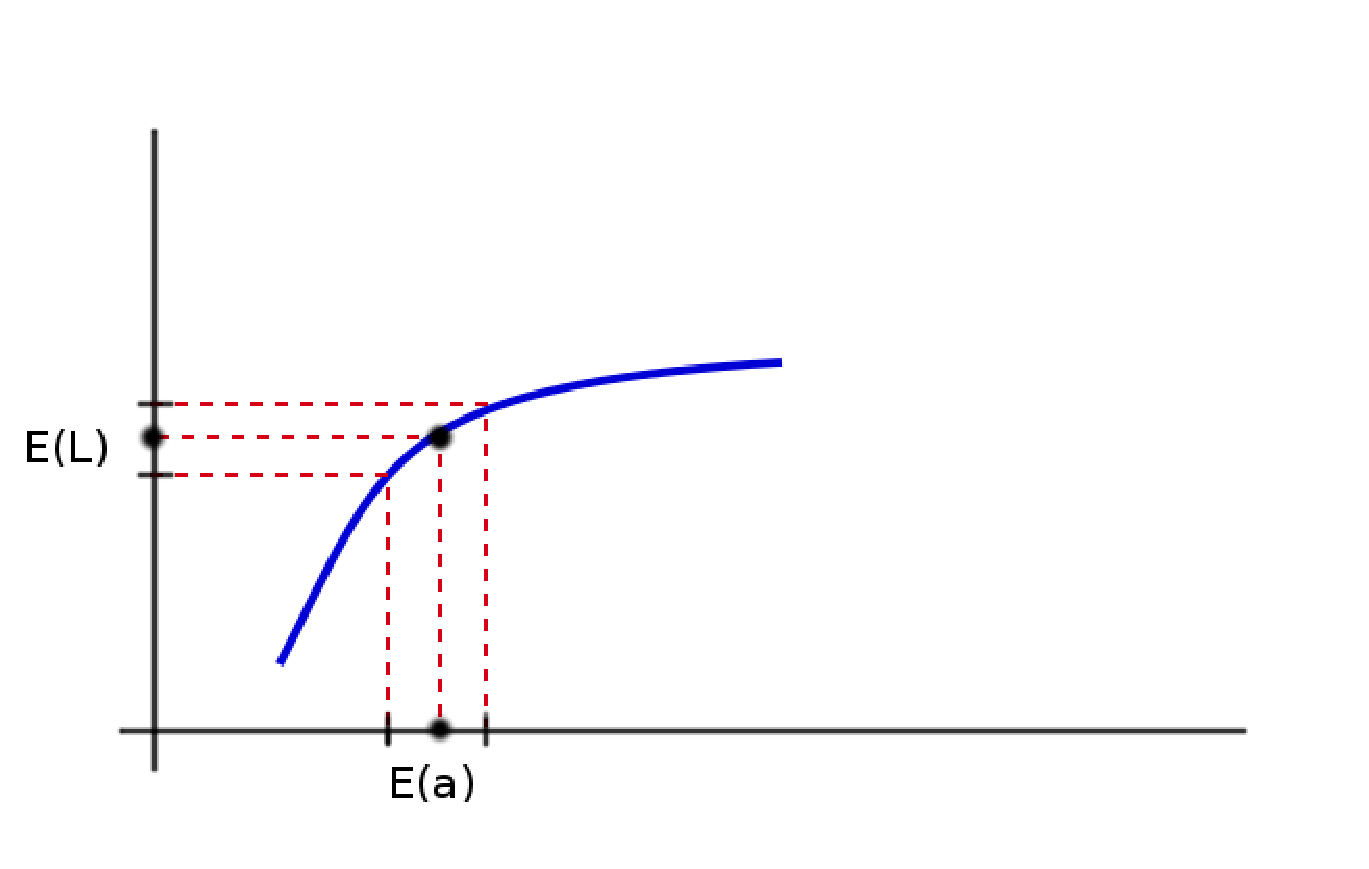
\includegraphics[height=6cm,width=6cm]{limite01.eps}
\end{center} 
\end{minipage}
\begin{minipage}{.50\textwidth}
Continuando...\\

Decimos que el limite de la funcion f cuando $x$ tiende a $a$ ($x$ se acerca a $a$) es igual a $L$ y se nota:
	$$ \lim_{x \rightarrow a}{f(x)} = L $$
\end{minipage}
\hfill \\\\
$\odot$ La fucnion $f$ deve estar al menos definida en $\stackrel{\circ}{E}(L)$\\
$\odot$ $E(L)$ depende de $E(a)$\\

Para poder trabajar se utiliza la siguiente definicion formal:

$$ \lim_{x \rightarrow a}{f(x)} = L   \Leftrightarrow   \forall \varepsilon >0, \exists \delta (\varepsilon) >0 /  0 < |x-a|< \delta \Leftarrow |f(x) - L| < \varepsilon $$

Esto es: El limite de $f(x)$ con $x$ tendiendo a $a$ es $L$ si y solo si  para todo $\varepsilon$ positivo, existe un $\delta$ en fucnion de $\varepsilon$ tal que el entorno reducido de centro $a$ y radio $\delta$ implicque que el valor absoluto de la resta de $f(x)$ menos $L$ sea menor a $\varepsilon$.\\

En si plantea que si evaluamos $f(x)$ en puntos cercanos a $a$, la funcion devolvera valores cercanos a $L$ que estaran edentro del entorno $E(L)$.

\subsubsection{Ejemplo de limite sensillo}
$$\lim_{x\rightarrow 2}{2x +1 =7}$$
Demostraremos eso:
$$ \forall \varepsilon > 0, \exists \delta (\varepsilon) >0 / 0<|x-3|<\delta \Rightarrow |(2x+1)- 7|<\varepsilon$$
Dado un $\varepsilon > 0$ (fijamos un $\varepsilon$ para poder trabajar).

$$ |(2x+1)-7| < \varepsilon \Rightarrow |2x+1-7| < \varepsilon \Rightarrow\ |2 \times (x-3)|< \varepsilon \Rightarrow 2 \times \underbrace{|x-3|}_{< \delta}< \varepsilon $$
$$ |x-3|< \delta \Rightarrow 2\delta < \varepsilon \Rightarrow \delta = \frac{\varepsilon}{2}$$
$\therefore$ Dado $\varepsilon>0, \exists \delta= \frac{\varepsilon}{2}$ tal que:
\begin{center}
$0<|x-3| < \frac{\varepsilon}{2} \Rightarrow 2(x-3)< \varepsilon       $  $ $ \checkmark demostrado.
\end{center}

\subsubsection{Pincipio de arquimedes}

Cada segmento ($y$) tan largo como se quiera puede ser cubiertos con un numero finito ($n$) de segmentos de longitud positiva tan pequenios como se quiera ($x$).
\begin{center}
\begin{pspicture}(0,0)(10,0.4)
\psaxes[labels=none]{-}(7,0)
\psdot(0.3,0)\rput[255](0.3,0.3){$x$}
\rput[255](0,-0.3){$0$}
\psdot(4,0)\rput[255](4,0.3){$y$}
\psdot(4.2,0)\rput[255](4.2,-0.4){$\overbrace{x\times n}$} 
\end{pspicture}\\ 
\end{center}

$$0<x<y<x\times n$$

\paragraph{Propiedad}
	Si tres nuemros reales $x$,$y$,$a$ satisfacen.
		$$ a \leq x \leq a + \frac{y}{n}  \forall n \in \mathbb{N}; x,y,a \in \mathbb{R}$$
		$$\therefore x=a$$
\subparagraph{Demostracion}

Hip: $a\geq 0$, $x>0$, $y>0$, $n>0$

Sup: $a<x$, $x>0$, $x-a>0$

Usando el principio de arquimedes, $x=x-a>0$
\begin{center}
$n\times (x-a)>y \Rightarrow x-a > \frac{y}{n} \Rightarrow $\\
$\Rightarrow x>a+\frac{y}{n} \leftarrow ABSURDO!!$\\
(Ya que $ a\leq a + \frac{y}{n}$)\\
\end{center}

Llegando a un absurdo mostramos que la supocicion es falsa($a<x$), por tanto deve ser $a=x$. 

\subsection{Unicidad de limite}

$$\lim_{x\rightarrow a}{f(x)}=L1 \wedge \lim_{x\rightarrow a}{f(x)}=L2 \Rightarrow L1=L2$$
\paragraph{Demostracion}

Hip:

• $\lim_{x \rightarrow a}{f(x)}=L1 \Leftrightarrow \forall \varepsilon >0, \exists \delta _1 (\varepsilon) / 0<|x-a|<\delta _1 \Rightarrow |f(x)-L1|<\varepsilon$

• $\lim_{x \rightarrow a}{f(x)}=L2 \Leftrightarrow \forall \varepsilon >0, \exists \delta _2 (\varepsilon) / 0<|x-a|<\delta _2 \Rightarrow |f(x)-L2|<\varepsilon$\\

Si tomamos un $\delta = \min {\delta _1, \delta _2}$ entonces nos queda:

Dado un $\varepsilon>0$, $\delta$
$$0<|x-a|<\delta \Rightarrow |f(x)-L1|<\varepsilon \wedge |f(x)-L2|<\varepsilon$$
\begin{center}
\fbox{
$a>0$, $b>0$, $c>0$ $\in \mathbb{R} \Rightarrow
\left.
\begin{array}{ccc}
a &<& c\\
b &<& c\\
\end{array}\right\} \Rightarrow a+b < c+c$}
\end{center}
$$\Rightarrow |f(x)-L1|+|f(x)-L2| < \varepsilon + \varepsilon \Rightarrow |f(x)-L1|-|f(x)-L2|<|f(x)-L1|+|f(x)-L2|< 2\varepsilon \Rightarrow$$
$$\Rightarrow |f(x)-L1-(f(x)-L2)|<2\varepsilon \Rightarrow |f(x)-L1-(f(x)-L2)|<2\varepsilon \Rightarrow$$
$$\Rightarrow |f(x)-L1- f(x)+L2|< 2\varepsilon \Rightarrow |L2-L1|< 2\varepsilon$$

En base a la propiedad del \textbf{Pincipio de Arquimedes}.
\begin{center}
\fbox{$a\leq x\leq a+ \frac{y}{n} \Rightarrow a=x$, donde $a$, $x$, $y$ $\in \mathbb{R}$ y $n \in \mathbb{N}$}
\end{center}

Tomando $a=0$, $x=|L2-L1|$, $\varepsilon=\frac{1}{2n}$ resulta:
$$0\leq |L2-L1|\leq 0+ 2\times \frac{1}{2n} \Rightarrow 0\leq |l2-l1|\leq \frac{1}{n} \Rightarrow 0=|L2-L1|\Rightarrow 0=L2-L1 \Rightarrow L2=L1 $$
\begin{center}
Son el mismo limite!
\end{center}

\subsection{Caracter local de limite}

Sean $f$ y $g$ dos funciones definidas en un $\stackrel{\circ}{E}(a)$ de manera que $\exists \delta >0 /$ \\ $ f(x)=g(x), \forall x/0<|x-a|<\delta$ entonces los limites de $f(x)$ y $g(x)$ con $x\rightarrow a$ son el mismo.

\paragraph{Demostracion} 


$$\lim_{x\rightarrow a}{f(x)}=L \Leftrightarrow \forall \varepsilon>0, \exists \delta _1 (\varepsilon)>0/0<|x-a|< \delta _1 \Rightarrow |f(x)-L|\varepsilon$$

Como por hipotesis $f(x)=g(x)$ $\forall x\in \stackrel{\circ}{E}(a,\delta _1)$. Tomo el minimo: $\delta _2 = \min {\delta _1 , \delta}$ ($\delta$ hipotesis).

Seguimos, dado $\varepsilon>0, \exists \delta _2/$
$$0<|x-a|\delta _2 \Rightarrow |f(x)-L|< \varepsilon \stackrel{\stackrel{en 0<|x-a|<\delta _2}{f(x)=g(x)}}{\Rightarrow} |g(x)-L<\varepsilon$$

Entonces dado $\varepsilon, \exists \delta _2 $
$$/ 0<|x-a|<\delta _2 \Rightarrow |g(x)-L|<\varepsilon \Leftrightarrow \lim_{x \rightarrow a}{g(x)}=L$$

$$\therefore \lim_{x \rightarrow a}{f(x)}=L =\lim_{x \rightarrow a}{g(x)}$$

\subsection{Formulas equivalentes}

\paragraph{1)}
$$\lim_{x \to a}{f(x)}=L \Leftrightarrow \lim_{x \to a}{f(x)-L}=0 \Leftrightarrow \lim_{x \to a}{|f(x)-L|}=0$$
 
\subparagraph{Demostracion \\}

$$\lim_{x \to a}{f(x)} =L\Leftrightarrow \forall \varepsilon >0, \exists \delta (\varepsilon)>0/ 0<|x-a|<\delta \Rightarrow |f(x)-L|<\varepsilon \Leftrightarrow$$
$$\Leftrightarrow 0<|x-a|<\delta \Rightarrow |f(x)-L|=|(f(x)-L)-0| <\varepsilon \Leftrightarrow \lim_{x \to a}{f(x)-L}=0 \Leftrightarrow$$
\fbox{$||x||=|x|$(propiedade de valor absoluto)}
$$\Leftrightarrow 0<|x-a|<\delta \Rightarrow |f(x)-L|=||(f(x)-L)-0|| <\varepsilon \Leftrightarrow \lim_{x \to a}{f(x)-L} = 0 $$

\paragraph{2) "Cambio de variable"}

$$\lim_{x \to a}{f(x)}=L \Leftrightarrow \lim_{h \to 0}{f(a+h)-L}=0 $$

\subparagraph{Demostracion \\ }

$$ \lim_{x \to a}{f(x)}=L \Leftrightarrow \forall \varepsilon >0, \exists \delta(\varepsilon)>0 / 0<|x-a|<\delta \Leftarrow |f(x)-L|< \varepsilon \Leftrightarrow$$
\begin{center}
  Defino $h=x-a$, $h=h-0$, despejo $x=a+h$ y sustituyo en la formula original quedando:
\end{center}
$$\Leftrightarrow 0<|h-0|<\delta \Leftarrow |f(a+h)-L| < \varepsilon \Leftrightarrow \lim_{h \to 0 }{f(a+h)}=L$$

\subsection{Teorema: "funcion acotada"}

Sea una funcion $f(x)$ con limite $L$ y vale $m<L<M$ entonces existe $\delta$ tal que $x\in \stackrel{\circ}{E}(a)$, $f(x)$ estara acotada inferiormente por $m$ y superiormente por $M$.

$$\lim_{x \to a}{f(x)}=L \wedge m<L<M \Rightarrow [\exists \delta >0/0<|x-a|<\delta \Rightarrow m<f(x)<M]$$

\paragraph{Demostracion \\}

Supuesto: $\lim_{x \to a}{f(x)}=L \wedge m<L<M$

